\documentclass{article}

\usepackage[latin1]{inputenc}
\usepackage{tikz}
\usetikzlibrary{calc}
\usepackage{tkz-euclide}
\tikzset{line/.style={draw, thick, -latex'}}
%\usetikzlibrary{shapes,arrows}
\begin{document}
\pagestyle{empty}


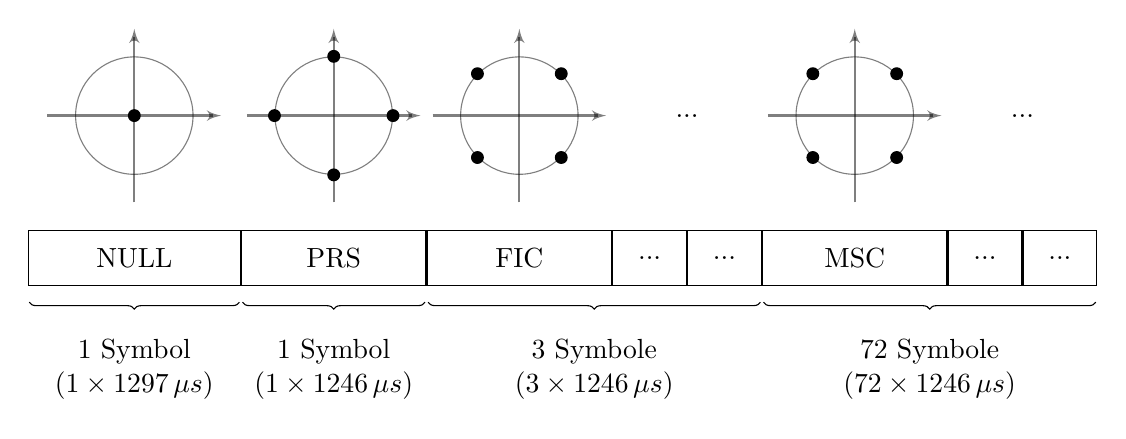
\begin{tikzpicture}[node distance = 0.5cm, auto]
\tikzstyle{block} = [rectangle, rounded corners, draw, text width=6em, text centered, minimum height=2em]
\tikzstyle{rect} = [rectangle, draw, text width=6em, text centered, minimum height=2em]
\tikzstyle{input} = [rectangle, text width=2em, align=right, minimum height=2em]
\tikzstyle{ci} = [circle, draw, inner sep=1.5em, opacity=0.5]
\tikzstyle{cii} = [circle, fill, draw, inner sep=0.15em]

\node [rect, text width=7em](null){NULL};
\node [rect, right=0.0cm of null.east](pilot){PRS};
\node [rect, right=0.0cm of pilot.east](fic1){FIC};
\node [rect, right=0.0cm of fic1.east, text width=2em](fic2){...};
\node [rect, right=0.0cm of fic2.east, text width=2em](fic3){...};
\node [rect, right=0.0cm of fic3.east](cif1){MSC};
\node [rect, right=0.0cm of cif1.east, text width=2em](cif2){...};
\node [rect, right=0.0cm of cif2.east, text width=2em](cif3){...};

% geschweifte klammern
\draw[-,decorate,decoration=brace] 
    ($(null.south east)+(-0.2mm,-2mm)$) -- ($(null.south west)+(0.2mm,-2mm)$) node [midway, yshift=-0.3cm]{\begin{tabular}{cc}
1 Symbol \\
($1\times 1297\, \mu s $)
\end{tabular}};
\draw[-,decorate,decoration=brace] 
    ($(pilot.south east)+(-0.2mm,-2mm)$) -- ($(pilot.south west)+(0.2mm,-2mm)$) node [midway, yshift=-0.3cm]{\begin{tabular}{cc}
1 Symbol \\
($1\times 1246\, \mu s $)
\end{tabular}};
\draw[-,decorate,decoration=brace] 
    ($(fic3.south east)+(-0.2mm,-2mm)$) -- ($(fic1.south west)+(0.2mm,-2mm)$) node [midway, yshift=-0.3cm]{\begin{tabular}{cc}
3 Symbole \\
($3\times 1246\, \mu s $)
\end{tabular}};
\draw[-,decorate,decoration=brace] 
    ($(cif3.south east)+(-0.2mm,-2mm)$) -- ($(cif1.south west)+(0.2mm,-2mm)$) node [midway, yshift=-0.3cm]{\begin{tabular}{cc}
72 Symbole \\
($72\times 1246\, \mu s $)
\end{tabular}};

% circles
\node [ci, above=0.7cm of null.north](c1){};
	\node [cii](c11) at (c1) {};
	\draw [line, opacity=0.5] ($(c1.south)+(0.0,-3.5mm)$)--($(c1.north)+(0.0,3.5mm)$);
	\draw [line, opacity=0.5] ($(c1.west)+(-3.5mm,0.0)$)--($(c1.east)+(3.5mm,0.0)$);
	
\node [ci, above=0.7cm of pilot.north](c2){};
	\node [cii](c21) at (c2.0) {};
	\node [cii](c22) at (c2.90) {};
	\node [cii](c23) at (c2.180) {};
	\node [cii](c24) at (c2.270) {};
	\draw [line, opacity=0.5] ($(c2.south)+(0.0,-3.5mm)$)--($(c2.north)+(0.0,3.5mm)$);
	\draw [line, opacity=0.5] ($(c2.west)+(-3.5mm,0.0)$)--($(c2.east)+(3.5mm,0.0)$);
	
\node [ci, above=0.7cm of fic1.north, anchor=south](c2){};
	\node [cii](c21) at (c2.45) {};
	\node [cii](c22) at (c2.135) {};
	\node [cii](c23) at (c2.225) {};
	\node [cii](c24) at (c2.315) {};
	\draw [line, opacity=0.5] ($(c2.south)+(0.0,-3.5mm)$)--($(c2.north)+(0.0,3.5mm)$);
	\draw [line, opacity=0.5] ($(c2.west)+(-3.5mm,0.0)$)--($(c2.east)+(3.5mm,0.0)$);
\node [above=1.45cm of fic2.north east, anchor=center](.1){...};

\node [ci, above=0.7cm of cif1.north, anchor=south](c2){};
	\node [cii](c21) at (c2.45) {};
	\node [cii](c22) at (c2.135) {};
	\node [cii](c23) at (c2.225) {};
	\node [cii](c24) at (c2.315) {};
	\draw [line, opacity=0.5] ($(c2.south)+(0.0,-3.5mm)$)--($(c2.north)+(0.0,3.5mm)$);
	\draw [line, opacity=0.5] ($(c2.west)+(-3.5mm,0.0)$)--($(c2.east)+(3.5mm,0.0)$);
\node [above=1.45cm of cif2.north east, anchor=center](.1){...};

\end{tikzpicture}
\end{document}